\subsection{Der Logger-Dialog}
Die Kommunikation mit dem Logger wird durch den Logger-Dialog erm�glicht. In diesem Dialog sind alle Funktionen enthalten, die notwendig sind, um Daten vom Logger zu lesen oder auf den Logger zu laden.
Diesen Dialog ruft man �ber das Men� ''Datei'' mit dem Eintrag ''Logger �ffnen'' auf. 

\subsubsection{Logger mit dem Computer verbinden}
Um die Daten aus einem Logger zu lesen, wird der Logger in der Regel durch ein Datenkabel mit dem Computer verbunden.
\\Nach dem �ffnen des Loggerdialoges gelangt man zuerst zu dem Teil des Dialoges, in dem die Einstellungen vorgenommen werden k�nnen.
Hier kann nun der Logger und die Schnittstelle, �ber die der Logger mit dem Computer verbunden ist, eingestellt werden.
\begin{figure}[htpb]
\begin{center}
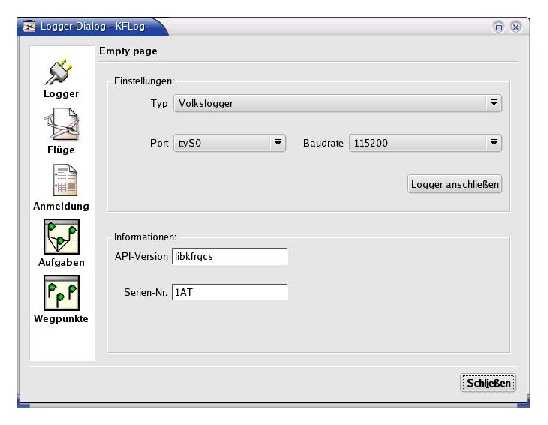
\includegraphics[scale=1]{Bilder/fertig/Loggerdialog.ps} 
\\
\caption{Verbindung mit einem Logger}
\end{center}
\end{figure}
Z.Z. werden die Logger vom Typ Volkslogger,Filser und Garmin unterst�tzt.
Weiterhin ist es m�glich Fl�ge, die mit dem Cumulus-System (http://cumulus.kflog.org/) aufgezeichnet worden sind, einzulesen.
\\Der Verbindungsaufbau erfolgt im wesentlichen in 3 Schritten:
\begin{enumerate}
\item Verbindungskabel an den Computer anschlie�en
\item Im Loggerdialog die Schnittstelle konfigurieren und den Logger ausw�hlen
\item Anschlie�en des Loggers an das Kabel und dr�cken des Knopfes ''Logger anschlie�en''
\end{enumerate}
Auf dem Logger sollte die entsprechende Meldung auf dem Display zu lesen sein, z.B. erscheint bei einem Volkslogger dann die Meldung ''data-transfer ready!'' auf dem Display. Damit ist die Konfiguration abgeschlossen und das System ist zum Datenaustausch bereit.
\subsubsection{Fl�ge aus dem Logger lesen}
Durch Klick auf das Symbol mit der Bezeichnung ''Fl�ge'' wird der Einlesedialog aufgerufen.
Hier kann man zun�chst eine Liste mit allen auf dem Logger aufgezeichneten Fl�gen laden, indem man den Knopf ''Liste Laden'' bet�tigt.
\begin{figure}[htpb]
\begin{center}
\includegraphics[scale=1]{Bilder/fertig/Loggerdialog-Fl�ge.ps} 
\\
\caption{Loggerdialog-Fl�ge}
\end{center}
\end{figure}
\\Diese Liste wird dann in einer �bersicht, chronologisch geordnet, angezeigt (s. Abb. 29). 
Nun kann der gew�nschte Flug mit der Maus markiert und vom Logger gelesen werden (Klick auf ''Flug sichern''), wobei eine IGC-Datei erzeugt wird.
Diese Datei wird im Verzeichnis f�r die Fl�ge abgelegt.
\subsubsection{Aufgaben in den Logger laden}
Um f�r eine Aufgabe die maximal m�gliche Punktzahl zu erhalten, ist es notwendig, den Flug vor Beginn zu deklarieren, d.h. die Anmeldung und die Aufgabe m�ssen vor dem Start an den Logger �bermittelt werden.
\\Die Anmeldung erfolgt im Loggerdialog indem man auf das Symbol Anmeldung klickt.
In diesem Dialog kann man die Aufgabe ausw�hlen (diese Aufgabe muss vorher erstellt bzw. in KFlog eingeladen worden sein). Die Ausgew�hlte Aufgabe wird als �bersicht mit den Wendepunkten und der Entfernung angezeigt. Vor dem �bertragen sind im untereren Bereich noch die Namen der Piloten sowie die Wettbewerbsklasse in die freien Felder einzutragen und der Flugzeugtyp ist einzustellen.
\\Anschlie�end kann der Knopf ''Anmeldung an Logger �bertragen'' geklickt werden und die Daten werden in den Logger transferiert. Anschlie�end kann am Logger �berpr�ft werden, ob die Daten ordnungsgem�� im Logger ''angekommen'' sind.
\begin{figure}[htpb]
\begin{center}
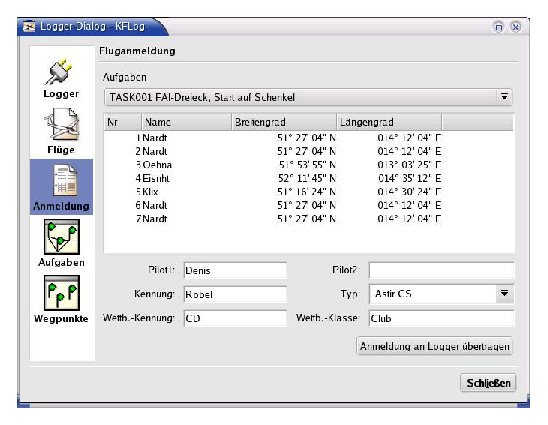
\includegraphics[scale=1]{Bilder/fertig/Loggerdialog-Anmeldung.ps} 
\\
\caption{Anmeldung einer Aufgabe in den Logger}
\end{center}
\end{figure}  

